\documentclass[12pt,a4paper]{article}
\usepackage[utf8]{inputenc}
\usepackage{amsmath}
\usepackage{amsfonts}
\usepackage{amssymb}
\usepackage{graphicx}
\usepackage{xcolor}
\usepackage{tikz}
\usepackage{pgfplots}
\pgfplotsset{compat=1.18}
\usepackage[left=2cm,right=2cm,top=2cm,bottom=2cm]{geometry}
\usepackage{enumitem}

% Bobot adalah subtotal; poin adalah nilai untuk langkah yang dinilai.
\newcommand{\bobot}[1]{\mbox{\textcolor{red}{\textbf{(#1 poin)}}}}
\newcommand{\poin}[1]{\mbox{\textcolor{red}{\textbf{[#1 poin]}}}}

\begin{document}

\begin{center}
  \textbf{\Large KUIS ke 1}\\[0.5cm]
  \textbf{\large Waktu : 90 menit}
\end{center}
\vspace{0.5cm}

\begin{enumerate}
  \item Dapatkan himpunan penyelesaian dari pertidaksamaan berikut
        \bobot{20}:
        \[
          \frac{x^2-16}{(x-1)^2}<0
        \]

  \item Dapatkan himpunan penyelesaian dari nilai mutlak berikut
        \bobot{20}:
        \[
          \sqrt{9x^2+6x+1}\geq 5
        \]

  \item Diketahui persamaan garis $10y+3x=-2$ \bobot{30}:
        \begin{enumerate}[label=\alph*.]
          \item Sketsalah grafik persamaan garis tersebut.
          \item Tentukan persamaan garis yang tegak lurus dengannya dan melalui titik $(8,2)$.
        \end{enumerate}

  \item Diketahui $f(x)=x-4$ dan $g(x)=|x^2-1|$ \bobot{30}:
        \begin{enumerate}[label=\alph*.]
          \item Dapatkan $(f\circ g)(x)$.
          \item Tentukan domain dan range $f\circ g(x)$.
          \item Sketsalah grafik $f\circ g(x)$.
        \end{enumerate}
\end{enumerate}

\newpage
\begin{center}
  \textbf{\Large PEMBAHASAN DAN PENILAIAN}
\end{center}
\vspace{0.3cm}

\begin{enumerate}
  \item \bobot{20}

        Penyebut tidak boleh nol, sehingga
        \[
          (x-1)^2\neq 0\implies x\neq 1.
        \]
        Syarat ini mendapat \poin{4}.

        Untuk $x\neq 1$, penyebut $(x-1)^2$ selalu positif. Oleh karena itu,
        pecahan bernilai negatif jika pembilangnya negatif:
        \poin{4}
        \[
          x^2-16<0.
        \]
        Faktorkan pembilang:
        \[
          (x-4)(x+4)<0.
        \]
        Titik kritisnya adalah $x=-4$ dan $x=4$. Menentukan interval yang
        memenuhi pertidaksamaan ini mendapat \poin{4}:
        \[
          -4<x<4.
        \]

        Karena $x=1$ tidak termasuk domain, keluarkan nilai tersebut dari
        interval di atas. Langkah ini mendapat \poin{4}. Jadi, himpunan
        penyelesaiannya adalah \poin{4}
        \[
          \boxed{\mathrm{HP}=\{x\in\mathbb{R}\mid -4<x<1
          \text{ atau }1<x<4\}}
        \]
        atau
        \[
          \boxed{\mathrm{HP}=(-4,1)\cup(1,4)}.
        \]

  \item \bobot{20}

        Ubah bentuk akar menjadi nilai mutlak:
        \poin{4}
        \[
          \sqrt{9x^2+6x+1}
          =\sqrt{(3x+1)^2}=|3x+1|.
        \]
        Maka pertidaksamaannya menjadi
        \[
          |3x+1|\geq 5.
        \]

        Untuk $|u|\geq a$ dengan $a>0$, berlaku $u\geq a$ atau $u\leq-a$.
        Menerapkan aturan ini mendapat \poin{4}:
        \[
          3x+1\geq 5
          \quad\text{atau}\quad
          3x+1\leq -5.
        \]

        Kasus pertama:
        \poin{4}
        \[
          3x+1\geq 5
          \implies 3x\geq 4
          \implies x\geq \frac{4}{3}.
        \]
        Kasus kedua:
        \poin{4}
        \[
          3x+1\leq -5
          \implies 3x\leq -6
          \implies x\leq -2.
        \]

        Jadi, himpunan penyelesaiannya adalah \poin{4}
        \[
          \boxed{\mathrm{HP}=(-\infty,-2]\cup
          \left[\frac{4}{3},\infty\right)}.
        \]

  \item \bobot{30}

        \begin{enumerate}[label=\alph*.]
          \item \bobot{12} Untuk membuat sketsa, ubah persamaan ke bentuk
                gradien-intersep:
                \poin{4}
                \begin{align*}
                  10y+3x&=-2,\\
                  10y&=-3x-2,\\
                  y&=-\frac{3}{10}x-\frac{1}{5}.
                \end{align*}
                Jadi, gradien garis adalah $-\frac{3}{10}$ dan titik potong
                sumbu-$y$ adalah $(0,-\frac15)$. \poin{4}

                Titik potong sumbu-$x$ diperoleh ketika $y=0$:
                \[
                  3x=-2\implies x=-\frac23.
                \]
                Dengan demikian, garis melalui
                $\left(-\frac23,0\right)$ dan
                $\left(0,-\frac15\right)$. \poin{4}

                \begin{center}
                  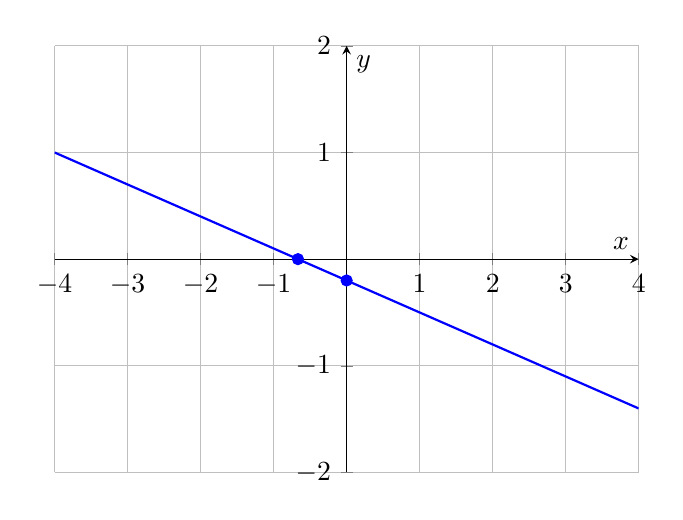
\begin{tikzpicture}
                    \begin{axis}[
                        axis lines=middle,
                        xlabel={$x$},
                        ylabel={$y$},
                        xmin=-4, xmax=4,
                        ymin=-2, ymax=2,
                        grid=both,
                        width=9cm,
                        height=7cm,
                        samples=2
                      ]
                      \addplot[domain=-4:4, thick, blue] {-3*x/10-1/5};
                      \addplot[mark=*, blue] coordinates
                        {(-2/3,0) (0,-1/5)};
                    \end{axis}
                  \end{tikzpicture}
                \end{center}

          \item \bobot{18} Gradien garis yang diketahui adalah
                $m_1=-\frac{3}{10}$. Untuk dua garis yang tegak lurus,
                hasil kali gradiennya adalah $-1$: \poin{5}
                \[
                  m_1m_2=-1
                  \implies -\frac{3}{10}m_2=-1
                  \implies m_2=\frac{10}{3}.
                \]

                Gunakan bentuk titik-gradien untuk garis melalui $(8,2)$:
                \poin{5}
                \[
                  y-2=\frac{10}{3}(x-8).
                \]
                Sederhanakan persamaan tersebut: \poin{4}
                \begin{align*}
                  3y-6&=10x-80,\\
                  \boxed{10x-3y-74=0}.
                \end{align*}
                \textit{(Bentuk ekuivalen, misalnya
                $y=\frac{10}{3}x-\frac{74}{3}$, juga benar.)}
                \poin{4}
        \end{enumerate}

  \item \bobot{30}

        \begin{enumerate}[label=\alph*.]
          \item \bobot{10} Komposisi fungsi diperoleh dengan memasukkan
                $g(x)$ ke dalam $f$:
                \poin{4}
                \begin{align*}
                  (f\circ g)(x)&=f(g(x))\\
                                &=f(|x^2-1|).
                \end{align*}
                Karena $f(t)=t-4$, maka \poin{3}
                \[
                  \boxed{(f\circ g)(x)=|x^2-1|-4}.
                \]
                Bentuk fungsi pecahannya adalah \poin{3}
                \[
                  (f\circ g)(x)=
                  \begin{cases}
                    -x^2-3, & -1\leq x\leq 1,\\
                    x^2-5, & x<-1\text{ atau }x>1.
                  \end{cases}
                \]

          \item \bobot{10} Domain $g$ adalah seluruh bilangan real karena
                $x^2-1$ terdefinisi untuk setiap $x\in\mathbb{R}$ dan nilai
                mutlak juga terdefinisi untuk setiap bilangan real.
                Fungsi $f$ juga terdefinisi untuk semua bilangan real.
                Jadi, domain komposisinya adalah \poin{4}
                \[
                  \boxed{D_{f\circ g}=\mathbb{R}}.
                \]

                Karena $|x^2-1|\geq 0$, nilai minimum komposisi terjadi
                ketika $|x^2-1|=0$, yaitu saat $x=\pm1$:
                \[
                  (f\circ g)(\pm1)=0-4=-4.
                \]
                Nilainya tidak terbatas ke atas, sehingga range-nya adalah
                \poin{6}
                \[
                  \boxed{R_{f\circ g}=[-4,\infty)}.
                \]

          \item \bobot{10} Grafik menggunakan bentuk pecahan:
                \poin{3}
                \[
                  h(x)=(f\circ g)(x)=
                  \begin{cases}
                    -x^2-3, & -1\leq x\leq 1,\\
                    x^2-5, & x<-1\text{ atau }x>1.
                  \end{cases}
                \]
                Titik pentingnya adalah
                $(-1,-4)$, $(0,-3)$, dan $(1,-4)$.
                Untuk $x<-1$ atau $x>1$, grafik berbentuk parabola yang
                terbuka ke atas; untuk $-1\leq x\leq1$, grafik berbentuk
                bagian parabola yang terbuka ke bawah. \poin{3}

                \begin{center}
                  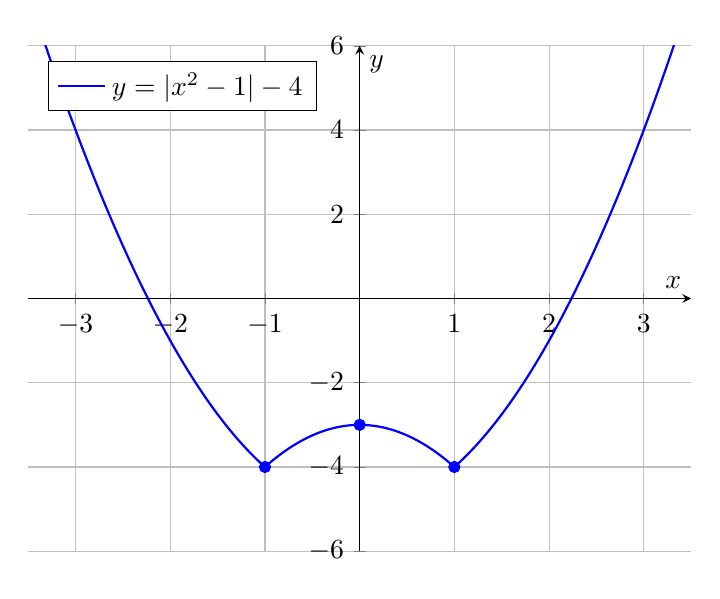
\begin{tikzpicture}
                    \begin{axis}[
                        axis lines=middle,
                        xlabel={$x$},
                        ylabel={$y$},
                        xmin=-3.5, xmax=3.5,
                        ymin=-6, ymax=6,
                        grid=both,
                        width=10cm,
                        height=8cm,
                        samples=100,
                        legend pos=north west
                      ]
                      \addplot[domain=-3.5:-1, thick, blue] {x^2-5};
                      \addplot[domain=-1:1, thick, blue] {-x^2-3};
                      \addplot[domain=1:3.5, thick, blue] {x^2-5};
                      \addlegendentry{$y=|x^2-1|-4$}
                      \addplot[only marks, mark=*, blue] coordinates
                        {(-1,-4) (0,-3) (1,-4)};
                    \end{axis}
                  \end{tikzpicture}
                \end{center}
                Sketsa yang benar dan mencantumkan titik penting mendapat
                \poin{4}.
        \end{enumerate}
\end{enumerate}

\end{document}